\documentclass{article}
\usepackage[paperwidth=6.5in,paperheight=1.8in,margin=0in]{geometry}
\usepackage{mathptmx}%{times}
\usepackage{graphicx}
\usepackage{siunitx}
\usepackage[absolute]{textpos}
\usepackage{color}
\usepackage{tikz}

\setlength{\parindent}{0pt}
\begin{document}
\TPMargin{1pt}
\begin{textblock}{0.75}(10.35,0.65)

\begin{tikzpicture}[
  scale=0.5
]
	\fill [orange!20] (0,0) rectangle (8.1,6.1);
\end{tikzpicture}
\end{textblock}
\begin{textblock}{4}(4.3,1.4)
\normalsize
$t = \SI{0}{\second}$
\end{textblock}
\begin{textblock}{4}(7.5,1.4)
\normalsize
$t = \SI{5000}{\second}$
\end{textblock}
\begin{textblock}{4}(11.5,1.4)
\normalsize
$t = \SI{10000}{\second}$
\end{textblock}
\centering
$z$ (\si{\meter}) \raisebox{-.5\height}{\includegraphics{../mountainAdvection-btf-5000-cubicUpwind-1000/10000/tracerContours.pdf}}
\begin{textblock}{5}(6.205,8.21)
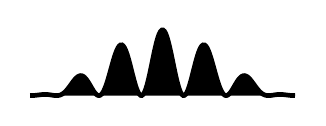
\begin{tikzpicture}[xscale=0.0673,yscale=0.167]
	\draw [fill=black,line width=1.7pt,domain=-25:25,samples=200] plot (\x,{5*cos(deg(\x*3.14159/8))*cos(deg(\x*3.14159/8))*cos(deg(\x*3.14159/50))*cos(deg(\x*3.14159/50))});
\end{tikzpicture}
\end{textblock}
\vspace*{0.3em}\hspace*{3.75em}$x$ (\si{\meter})
\end{document}
